\documentclass[10pt,a4paper]{article}
\usepackage[dvipsnames]{xcolor}
\usepackage[fleqn]{mathtools}
\usepackage{booktabs}
\usepackage{amsmath}
\usepackage{nccmath}
\usepackage{graphicx}
\usepackage{multicol}
\usepackage{listings}
\usepackage{tasks}
\usepackage{color}
\usepackage{float}
\usepackage[left=2cm,right=2cm,top=2cm,bottom=2cm]{geometry}

\begin{document}

\begin{titlepage}
	\centering
	{ \huge \scshape National Polytechnic Institute\par}
	{ \Large \scshape  Superior School of Computer Sciences\par }
	\vspace{1cm}
	{\scshape\Large Algorithm Analysis.\par}
	\vspace{1.5cm}
	{\huge\bfseries Practice 2 - Iterative vs Recursive Functions.\par}
	\vspace{2cm}
	{\Large\itshape Hernandez Martinez Carlos David. \\ Burciaga Ornelas Rodrigo Andres.\par} \hfill \break
	{\Large\itshape davestring@outlook.com. \\ andii\_burciaga@live.com.\par} \hfill \break
	{\Large\itshape Group: 3cv2. \par}
	\vfill
	{\large \today\par} 
	\vfill
\end{titlepage}

\renewcommand\lstlistingname{Quelltext} 

\lstset{ 
	language=Python,
	basicstyle=\small\sffamily,
	numbers=left,
 	numberstyle=\tiny,
	frame=tb,
	tabsize=4,
	columns=fixed,
	showstringspaces=false,
	showtabs=false,
	keepspaces,
	commentstyle=\color{lightgray},
	keywordstyle=\color{Violet} \bfseries,
	stringstyle=\color{MidnightBlue}
}

\settasks{
	counter-format=(tsk[r]),
	label-width=4ex
}

\tableofcontents 
\pagenumbering {arabic}
\pagebreak

\section{Introduction:}

Recurrences go hand in hand with the divide-and-conquer paradigm, because they
give us a natural way to characterize the running times of divide-and-conquer algorithms. A {\bfseries\itshape recurrence} is an equation or inequality that describes a function in terms of its value on smaller inputs. For example,  the worst-case running time \break {\bfseries\itshape T( n )} of the MERGE-SORT procedure by the recurrence: 

\begin{ceqn}
\begin{align}
T( n ) = \left\{
\begin{array}{ll}
\theta ( 1 ) & \mathrm {if\ } n = 1 \\
2T(\frac{n}{2}) + \theta ( n ) & \mathrm {if\ } n > 1 \\
\end{array}
\right.
\end{align}
\end{ceqn} 

whose solution claimed to be {\bfseries\itshape T( n ) = $\theta ( nlog( n ) )$}. \hfill \break

Recurrences can take many forms. For example, a recursive algorithm might divide subproblems into unequal sizes, such as a $\frac{2}{3}-to-\frac{1}{3}$ split.  If the divide and combine steps take linear time, such an algorithm would give rise to the recurrence: T( n ) = $T(\frac{2n}{3}) + T(\frac{n}{3}) + \theta ( n )$. \hfill \break

Sub-problems are not necessarily constrained to being a constant fraction of the original problem size. For example, a recursive version of linear search would create just one sub-problem containing only one element
fewer than the original problem. Each recursive call would take constant time plus the time for the recursive calls it makes, yielding the recurrence: T( n ) = $T( n - 1) + \theta ( 1 )$. \hfill \break

For solving recurrences the following methods are used:

\begin{itemize}
\item {\bfseries\itshape Substitution method}: We guess a bound and then use mathematical induction
to prove our guess correct.
\item {\bfseries\itshape Recursion-tree method}: Converts the recurrence into a tree whose nodes represent the costs incurred at various levels of the recursion. We use techniques for bounding summations to solve the recurrence.
\item {\bfseries\itshape Master method}: Provides bounds for recurrences of the form:

\begin{ceqn}
\begin{align}
T(n) = aT(\frac{n}{b}) + f(n) \ where\ a\ \geq 1\,\ and\ b\ >\ 1. 
\end{align}
\end{ceqn}
\end{itemize}

Such recurrences arise frequently. A recurrence of the form in equation (2) characterizes a divide-and-conquer
algorithm that creates {\bfseries\itshape a} sub-problems, each of which is {\bfseries\itshape $\frac{1}{b}$} the
size of the original problem, and in which the divide and combine steps together take {\bfseries\itshape f( n )} time.

\pagebreak

\section{Basic Concepts:}

When the sub-problems are large enough to solve recursively, we call that the {\bfseries\itshape recursive case}. Once the sub-problems become small enough that we no longer recurse, we say that the recursion “bottoms out” and that we have gotten down to the {\bfseries\itshape base case}. Sometimes, in addition to sub-problems that are smaller instances of the same problem, we have to solve sub-problems that are not quite the same as the original
problem. We consider solving such sub-problems as part of the combine step. 

\subsection{Divide-and-Conquer:}

The divide-and-conquer paradigm solve a problem recursively, applying three steps at each level of the recursion:

\begin{itemize}
\item {\bfseries\itshape Divide}: The problem into a number of sub-problems that are smaller instances of the
same problem.
\item {\bfseries\itshape Conquer}: The sub-problems by solving them recursively. If the sub-problem sizes are
small enough, however, just solve The sub-problems in a straightforward manner.
\item {\bfseries\itshape Combine}: The solutions to the sub-problems into the solution for the original problem.
\end{itemize}

\subsection{The Master Theorem:}

Let a $\geq$ 1 and b $>$ 1 be constants, let f( n ) be a function, and let T( n ) be defined
on the non-negative integers by the recurrence:

\begin{ceqn}
\begin{align}
T(n) = aT(\frac{n}{b}) + f(n)
\end{align}
\end{ceqn}

Then T( n ) has the following asymptotic bounds:

\begin{itemize}
\item If {\bfseries\itshape f( n )} = O ( $n^{log_{b}( a ) - \epsilon}\ )\ for\ some\ constant\ \epsilon\ >\ 0,\ then\ \theta\ (\ n^{log_{b}(\ a\ )}\ )$.
\item If {\bfseries\itshape f( n )} = $ \theta (\ n^{log_{b}( a )}\ ),\ then\ T(\ n\ )\ =\ \theta\ (\ n^{log_{b}(\ a\ )}\ lg(\ n\ )\ )$.
\item if {\bfseries\itshape f( n )} = $\Omega (\ n^{log_{b}( a ) + \epsilon}\ )\ for\ some\ constant\ \epsilon\ >\ 0$ and if {\bfseries\itshape f( $\frac{n}{b}\ )\ \leq$ cf( n )} for some constant $c\ <\ 1$ and all sufficiently large {\bfseries\itshape n}, then, T( n ) = $\theta (\ f(\ n\ )\ )$.
\end{itemize}
\pagebreak

\section{Development:}

\subsection{Fibonacci Algorithm:}

The Fibonacci program it's divided in 3 different modules:

\begin{itemize}
\item main.py: Control the sequence of execution.
\item fibonacci.py: Calculate and return a Fibonacci number F( n ). 
\item graph.py: Plot {\bfseries\itshape t} against {\bfseries\itshape F( n )}, where {\bfseries\itshape t} it's the time that takes to find the Fibonacci number {\bfseries\itshape F ( n )}.
\end{itemize}

{\bfseries\itshape\color{OliveGreen}{Observation:}} {\itshape\color{OliveGreen}{Fibonacci where programmed {\bfseries Recursive} and {\bfseries Iterative}, both algorithms are totally different, but {\bfseries main.py} and {\bfseries graph.py} are basically the same.}}

\subsubsection{Main.py}

In main.py, the program will ask the user to enter a number {\bfseries\itshape 'n'}, this number will be the parameter of the function {\bfseries\itshape fibonacci ( ... )}. After storing the returned values of {\bfseries\itshape fibonacci ( ... )}, the program will call \linebreak {\bfseries\itshape graph ( ... )} to plot {\bfseries\itshape time} against {\bfseries\itshape F( n ) = fibo}. \hfill \break

\begin{lstlisting}
def main ( ):
    n = -1
    while ( n <= 0 ):
        n = int ( input ( "\n\tFibonacci Number to Calculate: " ) )
    # fibonacci ( n ): Return the fibonacci number, the counter that takes to
    # find that number, and a list of the fibonacci numbers before 'fibo'.
    fibo, count, f = fibonacci ( n )
    print ( "\n\tFibonacci ( ", n, " ): ", fibo, "\n" )
    graph ( count, fibo, f, n )
main ( )
\end{lstlisting} 

\subsubsection{Graph.py}

For plotting the result I’m using {\bfseries\itshape matplotlib} and {\bfseries\itshape numpy}  and comparing the {\bfseries\itshape time ( t )}  determined by the counter returned in {\bfseries\itshape fibonacci ( ... )} and the ’list’ of the previous Fibonacci numbers after reaching \linebreak {\bfseries\itshape F( n ) = fibo} the program is able to plot the curve of the temporal complexity of the algorithm. \hfill \break

\begin{lstlisting}
def graph ( count, fibo, f, n ):
    # Window title.
    plt.figure ( "Fibonacci Iterative Algorithm" )
    # Graph title.
    plt.title ( "Fibonacci ( " + str ( n ) + " ): " + str ( fibo ) )
    # Parameter Time ( t ) and Fibonacci ( n ) of the graph.
    t = np.arange ( 0, count, ( count / ( len ( f ) + 1 ) ) )
    _t = list ( map ( ( lambda x: x * ( 3 / 2 ) ), t ) )
    _f = np.arange ( 0, len ( f ) + 1 )
    # Names of the axes.
    plt.xlabel ( "Time ( t )", color = ( 0.3, 0.4, 0.6 ), family = "cursive", 
    	size = "large" )
    plt.ylabel ( "Fibonacci ( f )", color = ( 0.3, 0.4, 0.6 ), family = "cursive", 
    	size = "large" )
    # Plot.
    plt.plot ( _f, t, "#778899", linewidth = 3, label = "T( n ) = ( ( n )" )
    plt.plot ( _f, _t, "#800000", linestyle = "--", label = "g( n ) = ( 3/2 )( n )" )
    plt.legend ( loc = "lower right" )
    plt.show ( )
\end{lstlisting} \pagebreak

\subsubsection{Fibonacci Iterative:}

The Fibonacci numbers are the numbers in the following integer sequence, called the Fibonacci sequence, and characterized by the fact that every number after the first two is the sum of the two preceding ones:

\begin{ceqn}
\begin{align}
1, 1, 2, 3, 5, 8, 13, 21, 34, 55, 89, 144, ...
\end{align}
\end{ceqn}

The code bellow, calculate a Fibonacci number where {\bfseries\itshape F( n ) = fibo} it's the Fibonacci number to find, {\bfseries\itshape F ( n - 1 ) = a} and {\bfseries\itshape F( n - 2 ) = b} are the two previous ones. \hfill \break

\begin{lstlisting}
def fibonacci ( n ):
	fibo, a, b = 0, 1, 0
    for i in range ( 1, n ):
        fibo = a + b
        b = a
        a = fibo
    return fibo
\end{lstlisting} \hfill

If we want to calculate the computational time {\bfseries\itshape T ( n )} that the algorithm takes to find a number, it's necessary to put a counter in each line of our code. \hfill \break

\begin{lstlisting}
def fibonacci ( n ):
    count, fibo, a, b, f = 1, 1, 1, 0, [ ]
    for i in range ( 1, n ):
        count += 1
        fibo = a + b
        count += 1
        f.append ( fibo )
        count += 1
        b = a
        count += 1
        a = fibo
        count += 1
    count += 1
    return fibo, count, f
\end{lstlisting} \hfill

{\bfseries\itshape\color{OliveGreen}{Observation:}} {\itshape\color{OliveGreen}{Now, apart of return the Fibonacci number result, the code will also return the counter and a list of all the previous Fibonacci numbers after 'n'.}} \hfill \break

{\bfseries\itshape\color{OliveGreen}{Observation:}} {\itshape\color{OliveGreen}{The counter and the list are necessary to plot {\bfseries t} against {\bfseries n} where {\bfseries t} it's the computation time.}}

\pagebreak

\subsubsection{Fibonacci Recursive:}

The sequence $F_{n}$ of Fibonacci numbers is defined by the recurrence relation:

\begin{ceqn}
\begin{align}
F_{n} = F_{n-1} + F_{n-2}
\end{align}
\end{ceqn}

with seed values:

\begin{ceqn}
\begin{align}
F_{n} = 1, F_{n} = 2
\end{align}
\end{ceqn} 

\begin{lstlisting}
def fibonacci ( n ):
    if ( n == 1 or n == 2 ):
        return 1
    else:
        return fibonacci ( n - 1 ) + fibonacci ( n - 2 )
\end{lstlisting} \hfill

For calculate the computation time of the algorithm it's necessary to modify some lines of the code: \hfill \break

\begin{lstlisting}
def fibonacci ( n, count ):
    count += 1
    if ( n == 1 or n == 2 ):
        return 1, count
    else:
        a, count = fibonacci ( n - 1, count )
        b, count = fibonacci ( n - 2, count )
        return a + b, count
\end{lstlisting} \hfill

As we can see, now the Fibonacci function receive two parameters, the 'n' and the counter to calculate the computational time, also in the {\bfseries\itshape else} sentence, the return of the recursions are stored in 3 variables {\bfseries\itshape a, b and counter} where {\bfseries\itshape a and b} are the two previous Fibonacci's. \hfill \break

The final return statement of the algorithm will be stored in main, were the Fibonacci function were initially called, and the values will be stored in a {\bfseries\itshape list of tuples}, where the values stored are {\bfseries\itshape ( F( n ), time )} where {\bfseries\itshape F( n )} it's the Fibonacci number and {\bfseries\itshape time} it's the computational time that the algorithm takes to find that number. For Example: n = 10.

\begin{figure}[H]
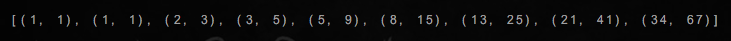
\includegraphics[scale=.65]{parameters.png}
\centering \linebreak \linebreak Figure 3.1.4.0: Return statement of Fibonacci recursive.
\end{figure}

According to the Figure 3.1.4.0:

\begin{center}
\begin{itemize}
\end{itemize}
\begin{tabular}[.5cm]{l c c }
\toprule
Fibonacci & Time \\
\midrule
1 & 1 \\
\cmidrule{1-2}
1 & 1 \\
\cmidrule{1-2}
2 & 3 \\
\cmidrule{1-2}
3 & 5 \\
\cmidrule{1-2}
5 & 9 \\
\cmidrule{1-2}
8 & 15 \\
\cmidrule{1-2}
21 & 41 \\
\cmidrule{1-2}
34 & 67 \\
\bottomrule
\linebreak
\end{tabular}
\linebreak Table 1: Fibonacci number against Computation Time.
\end{center}

\pagebreak

\subsection{Cube-Sum Algorithm:}

The Cube-Sum program it's divided in 3 different modules:

\begin{itemize}
\item main.py: Control the sequence of execution.
\item cube.py: Calculate and return a the sum of the nth numbers to the power '3': C ( n ). 
\item graph.py: Plot {\bfseries\itshape t} against {\bfseries\itshape C( n )}, where {\bfseries\itshape t} it's the time that takes to find the sum of the first nth numbers to the power '3' {\bfseries\itshape C ( n )}.
\end{itemize}

{\bfseries\itshape\color{OliveGreen}{Observation:}} {\itshape\color{OliveGreen}{Cube-Sum where programmed {\bfseries Recursive} and {\bfseries Iterative}, both algorithms are totally different, but {\bfseries main.py} and {\bfseries graph.py} are basically the same.}}

\subsubsection{Main.py:}

In main.py, the program will ask the user to enter a number {\bfseries\itshape 'n'}, this number will be the parameter of the function {\bfseries\itshape cube ( ... )}. After storing the returned values of {\bfseries\itshape cube ( ... )}, the program will call \linebreak {\bfseries\itshape graph ( ... )} to plot {\bfseries\itshape time} against {\bfseries\itshape C( n ) = sum}. \hfill \break

\begin{lstlisting}
def main ( ):
    n = int ( input ( "\n\tNumber to calculate firts n-Cubes: " ) )
    # cube ( n ): Return the _sum of the first 'n' cubes, the computational
    # time of the algorithm and a list of the sum of nth cubes.
    _sum, count, cubelist = cube ( n )
    print ( "\n\tThe sum of the first ", n, " cubes is: C ( ", n, " ) = ", _sum, "\n" )
    graph ( _sum, count, cubelist, n )
main ( )
\end{lstlisting}

\subsubsection{Graph.py:}

For plotting the result I’m using {\bfseries\itshape matplotlib} and {\bfseries\itshape numpy}  and comparing the {\bfseries\itshape time ( t )}  determined by the counter returned in {\bfseries\itshape cube ( ... )} and the ’list’ of the previous sum of nth cubes after reaching {\bfseries\itshape C( n ) = sum} the program is able to plot the curve of the temporal complexity of the algorithm. Also, in line 11, I propose a function g( n ) that T( n ) $\in$ O( g( n ) ) where T( n ) it's the computational time of the algorithm. \hfill \break

\begin{lstlisting}
def graph ( _sum, count, cubelist, n ):
    # Window title.
    plt.figure ( "First 'n' Cubes: Iterative Algorithm" )
    # Graph title.
    plt.title ( "CubeSum ( " + str ( n ) + " ): " + str ( _sum ) )
    # Parameter Time ( t ) of the graph.
    t = np.arange ( 0, count, ( count / ( len ( cubelist ) ) ) )
    # Parameter CubeSum ( n ) of the graph.
    c = np.arange ( 0, len ( cubelist ) )
    # Proposed function: g( n ) = ( 3/2 )n.
    _t = list ( map ( ( lambda x: x * ( 3 / 2 ) ), t ) )
    # Names of the axes.
    plt.ylabel ( "Time ( t )", color = ( 0.3, 0.4, 0.6 ), family = "cursive", 
    	size = "large" )
    plt.xlabel ( "CubeSum ( n )", color = ( 0.3, 0.4, 0.6 ), family = "cursive", 
    	size = "large" )
    # Plot.
    plt.plot ( c, _t, "#800000", linestyle = "--", label = "g( n ) = ( 3/2 )( n )" )
    plt.plot ( c, t, "#778899", linewidth = 3, label = "T( n ) = ( n )" )
    plt.legend ( loc = "lower right" )
    plt.show ( )
\end{lstlisting}

\pagebreak

\subsubsection{Cube-Sum Iterative:}

The Cube-Sum are the numbers in the following integer sequence, and characterized by the fact that every number its the sum of all the previous one to the power of '3'.

\begin{itemize}
\item Normal number to the power of '3' sequence:
\end{itemize}

\begin{ceqn}
\begin{align}
0, 1, 8, 27, 64, ...
\end{align}
\end{ceqn}

\begin{itemize}
\item Sum of the number to the power of '3' sequence:
\end{itemize}

\begin{ceqn}
\begin{align}
0, 1, 9, 36, 100, ...
\end{align}
\end{ceqn}

The code bellow, calculate the Cube-Sum of any number where {\bfseries\itshape C( n ) = sum} it's the sum result. \hfill \break

\begin{lstlisting}
def cube ( n ):
    _sum = 0
    # Range: From 1 <= i <= n.
    for i in range ( 1, n + 1 ):
        _sum = _sum + ( i * i * i )
    # Return statement.
    return _sum
\end{lstlisting} \hfill

If we want to calculate the computational time {\bfseries\itshape T ( n )} that the algorithm takes to find a number, it's necessary to put a counter in each line of our code. \hfill \break

\begin{lstlisting}
def cube ( n ):
    _sum, count, cubelist = 0, 1, [ ]
    # Range: From 1 <= i <= n.
    for i in range ( 1, n + 1 ):
        count += 1
        _sum = _sum + ( i * i * i )
        count += 1
        cubelist.append ( _sum )
        count += 1
    # Return statement.
    count += 1
    return _sum, count, cubelist
\end{lstlisting} \hfill

{\bfseries\itshape\color{OliveGreen}{Observation:}} {\itshape\color{OliveGreen}{Now, apart of return the sum result, the code will also return the counter and a list of all the previous numbers of the sequence after 'n'.}} \hfill \break

{\bfseries\itshape\color{OliveGreen}{Observation:}} {\itshape\color{OliveGreen}{The counter and the list are necessary to plot {\bfseries t} against {\bfseries n} where {\bfseries t} it's the computation time.}}

\pagebreak

\subsubsection{Cube-Sum Recursive:}

The sequence $C_{n}$ of Cube-Sum numbers is defined by the recurrence relation:

\begin{ceqn}
\begin{align}
C_{n} = C_{n-1} + ( n^{3} )
\end{align}
\end{ceqn}

with seed values:

\begin{ceqn}
\begin{align}
C_{n} = 1
\end{align}
\end{ceqn}

\begin{lstlisting}
def cube ( n ):
    if ( n == 1 ):
        return 1
    else:
        return cube ( n - 1 ) + ( n * n * n )
\end{lstlisting} \hfill

For calculate the computation time of the algorithm it's necessary to modify some lines of the code: \hfill \break

\begin{lstlisting}
def cube ( n, count ):
    count += 1
    if ( n == 1 ):
        return 1, count
    else:
        a, count = cube ( n - 1, count )
        b = n*n*n
        return a + b, count
\end{lstlisting} \hfill

As we can see, now the Cube function receive two parameters, the 'n' and the counter to calculate the computational time, also in the {\bfseries\itshape else} sentence, the return of the recursions are stored in 2 variables {\bfseries\itshape a and counter} where {\bfseries\itshape a} its the sum of the previous Cubes. \hfill \break

The final return statement of the algorithm will be stored in main, were the Cube function were initially called, and the values will be stored in a {\bfseries\itshape list of tuples} where the values stored are {\bfseries\itshape ( C( n ), time )} where {\bfseries\itshape C( n )} it's the Cube sum and {\bfseries\itshape time} it's the computational time that the algorithm takes to find that number. For Example: n = 10.

\begin{figure}[H]
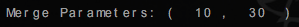
\includegraphics[scale=.55]{parameters1.png}
\centering \linebreak \linebreak Figure 3.2.4.0: Return statement of CubeSum recursive.
\end{figure}

According to the Figure 3.2.4.0:

\begin{center}
\begin{itemize}
\end{itemize}
\begin{tabular}[.5cm]{l c c }
\toprule
Cubesum & Time \\
\midrule
1 & 1 \\
\cmidrule{1-2}
9 & 2 \\
\cmidrule{1-2}
36 & 3 \\
\cmidrule{1-2}
100 & 4 \\
\cmidrule{1-2}
225 & 5 \\
\cmidrule{1-2}
441 & 6 \\
\cmidrule{1-2}
784 & 7 \\
\cmidrule{1-2}
1296 & 8 \\
\cmidrule{1-2}
2025 & 9 \\
\cmidrule{1-2}
3025 & 10 \\
\bottomrule
\linebreak
\end{tabular}
\linebreak Table 2: Cube sum against Computation Time.
\end{center}

\pagebreak

\section{Results:}

All the code shown above doesn't have significance if its operation is not shown. This section will show you the {\bfseries\itshape console} output and the graphic of the temporal complexity of the algorithms previously mentioned. Also, I attach a table with the plot points for each test.

\subsection{Fibonacci Iterative:}

First test of the Fibonacci Iterative Algorithm. The program will plot the {\bfseries\itshape time} that the algorithm takes to find the {\bfseries\itshape eight} Fibonacci number.

\begin{figure}[H]
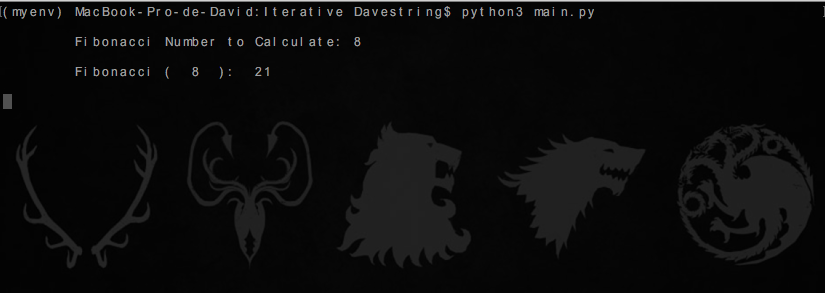
\includegraphics[scale=.6]{cfi1.png}
\centering \linebreak \linebreak Figure 4.1.0: Console output of Fibonacci Iterative.
\end{figure}

\begin{multicols}{2}
\begin{figure}[H]
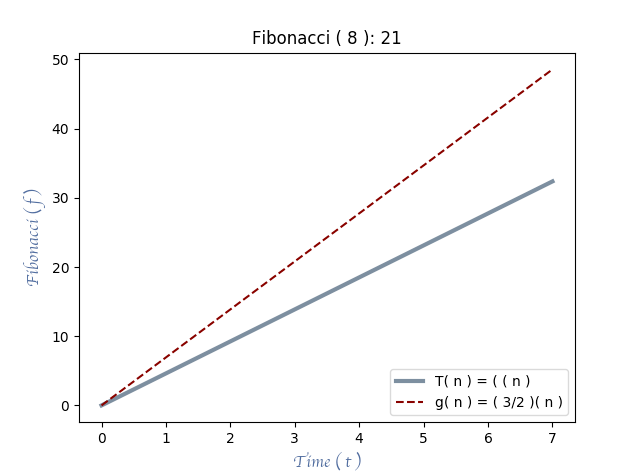
\includegraphics[scale=.4]{gfi1.png}
\centering \linebreak \linebreak Figure 4.1.1: Plot of Figure 4.1.0.
\end{figure}

\begin{center}
\begin{itemize}
\end{itemize}
\begin{tabular}[.5cm]{l c c }
\toprule
Time ( t ) & Fibonacci ( n ) \\
\midrule
0 & F ( 1 ) = 1 \\
\cmidrule{1-2}
4.80 & F ( 2 ) = 1 \\
\cmidrule{1-2}
9.60 & F ( 3 ) = 2 \\
\cmidrule{1-2}
14.40 & F ( 4 ) = 3 \\
\cmidrule{1-2}
19.20 & F ( 5 ) = 5 \\
\cmidrule{1-2}
24 & F ( 6 ) = 8 \\
\cmidrule{1-2}
28.80 & F ( 7 ) = 13 \\
\cmidrule{1-2}
33.60 & F ( 8 ) = 21 \\
\bottomrule
\linebreak
\end{tabular}
\linebreak Table 3: Plot points of Figure 4.1.1.
\end{center}
\end{multicols} \hfill

{\bfseries\itshape\color{OliveGreen}{Observation:}} {\itshape\color{OliveGreen}{The plot has two curves, the {\bfseries blue} one it's the computation time of our algorithm \linebreak {\bfseries T( n ) = n} and the {\bfseries red} one it's the proposed function {\bfseries g( n ) = $\frac{3}{2} n$}, where {\bfseries T( n ) $\in$ O ( g( n ) ).}}} \hfill \break

\pagebreak

Second test of the Fibonacci Iterative Algorithm. The program will plot the {\bfseries\itshape time} that the algorithm takes to find the {\bfseries\itshape fifteenth} Fibonacci number.

\begin{figure}[H]
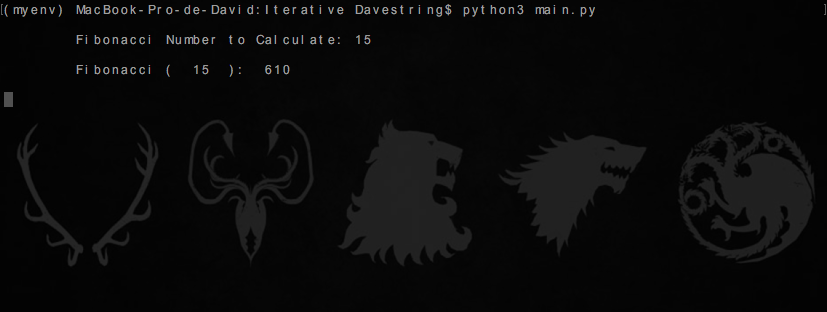
\includegraphics[scale=.6]{cfi2.png}
\centering \linebreak \linebreak Figure 4.1.2: Console output of Fibonacci Iterative.
\end{figure}

\begin{multicols}{2}
\begin{figure}[H]
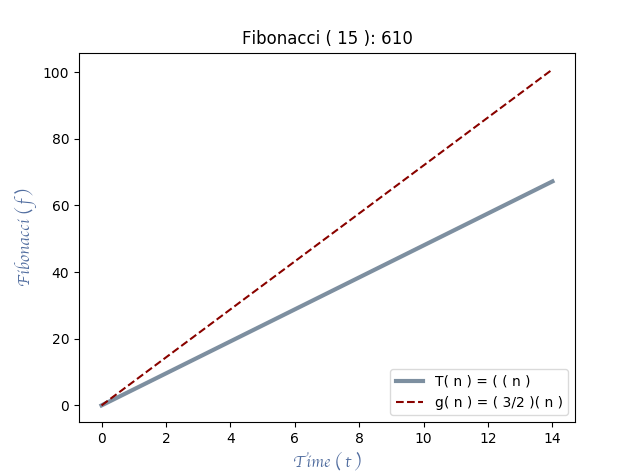
\includegraphics[scale=.4]{gfi2.png}
\centering \linebreak \linebreak Figure 4.1.3: Plot of Figure 4.1.2.
\end{figure}

\begin{center}
\begin{tabular}[.5cm]{l c c }
\toprule
Time ( t ) & Fibonacci ( n ) \\
\midrule
0 & F ( 1 ) = 1 \\
\cmidrule{1-2}
4.80 & F ( 2 ) = 1 \\
\cmidrule{1-2}
9.60 & F ( 3 ) = 2 \\
\cmidrule{1-2}
14.40 & F ( 4 ) = 3 \\
\cmidrule{1-2}
19.20 & F ( 5 ) = 5 \\
\cmidrule{1-2}
24 & F ( 6 ) = 8 \\
\cmidrule{1-2}
28.80 & F ( 7 ) = 13 \\
\cmidrule{1-2}
33.60 & F ( 8 ) = 21 \\
\cmidrule{1-2}
38.40 & F ( 9 ) = 34 \\
\cmidrule{1-2}
43.20 & F ( 10 ) = 55 \\
\cmidrule{1-2}
48 & F ( 11 ) = 89 \\
\cmidrule{1-2}
52.80 & F ( 12 ) = 144 \\
\cmidrule{1-2}
57.60 & F ( 13 ) = 233 \\
\cmidrule{1-2}
62.40 & F ( 14 ) = 377 \\
\cmidrule{1-2}
67.20 & F ( 15 ) = 610 \\
\bottomrule
\linebreak
\end{tabular}
\linebreak Table 4: Plot points of Figure 4.1.3.
\end{center}
\end{multicols} 

{\bfseries\itshape\color{OliveGreen}{Observation:}} {\itshape\color{OliveGreen}{As we can see, according to section 3.3 It is demonstrated that the algorithm is of linear order}}. 

\pagebreak

\subsection{Fibonacci Recursive:}

First test of the Fibonacci Recursive Algorithm. The program will plot the {\bfseries\itshape time} that the algorithm takes to find the {\bfseries\itshape eight} Fibonacci number.

\begin{figure}[H]
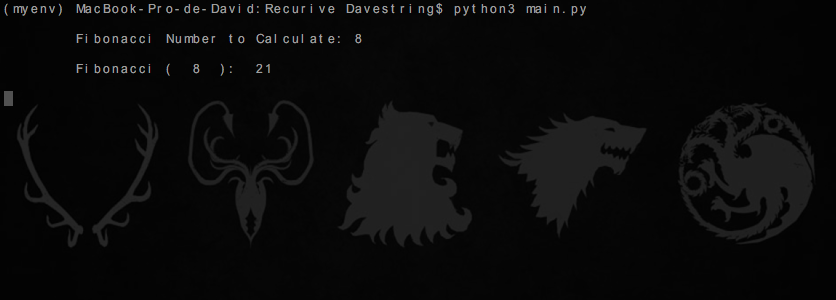
\includegraphics[scale=.6]{cfr1.png}
\centering \linebreak \linebreak Figure 4.2.0: Console output of Fibonacci Recursive.
\end{figure}

\begin{multicols}{2}
\begin{figure}[H]
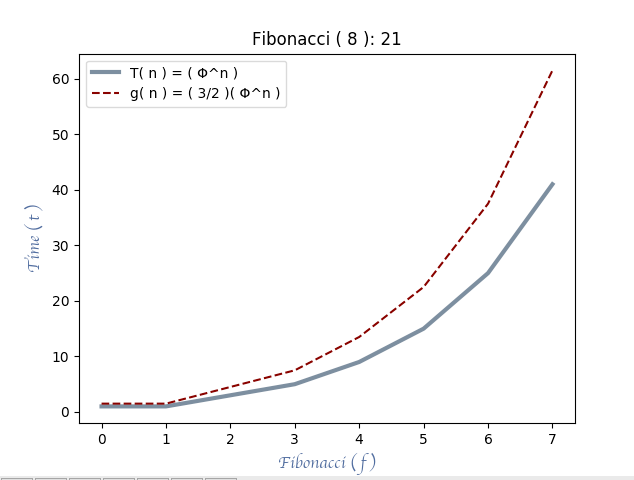
\includegraphics[scale=.4]{gfr1.png}
\centering \linebreak \linebreak Figure 4.2.1: Plot of Figure 4.2.0.
\end{figure}

\begin{center}
\begin{itemize}
\end{itemize}
\begin{tabular}[.5cm]{l c c }
\toprule
Time ( t ) & Fibonacci ( n ) \\
\midrule
1 & F ( 1 ) = 1 \\
\cmidrule{1-2}
1 & F ( 2 ) = 1 \\
\cmidrule{1-2}
3 & F ( 3 ) = 2 \\
\cmidrule{1-2}
5 & F ( 4 ) = 3 \\
\cmidrule{1-2}
9 & F ( 5 ) = 5 \\
\cmidrule{1-2}
15 & F ( 6 ) = 8 \\
\cmidrule{1-2}
25 & F ( 7 ) = 13 \\
\cmidrule{1-2}
41 & F ( 8 ) = 21 \\
\bottomrule
\linebreak
\end{tabular}
\linebreak Table 5: Plot points of Figure 4.2.1.
\end{center}
\end{multicols} \hfill

{\bfseries\itshape\color{OliveGreen}{Observation:}} {\itshape\color{OliveGreen}{The plot has two curves, the {\bfseries blue} one it's the computation time of our algorithm \linebreak {\bfseries T( n ) = ( $\phi^{n}$ )} and the {\bfseries red} one it's the proposed function {\bfseries g( n ) = $\frac{3}{2} ( \phi^{n} )$}, where {\bfseries T( n ) $\in$ O ( g( n ) ).}}} \hfill \break

\pagebreak

Second test of the Fibonacci Recursive Algorithm. The program will plot the {\bfseries\itshape time} that the algorithm takes to find the {\bfseries\itshape fifteenth} Fibonacci number.

\begin{figure}[H]
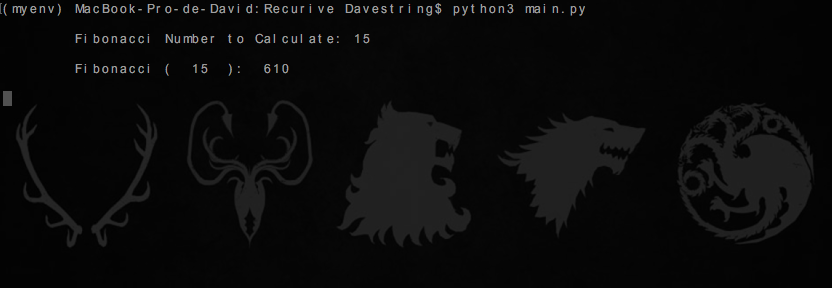
\includegraphics[scale=.6]{cfr2.png}
\centering \linebreak \linebreak Figure 4.2.2: Console output of Fibonacci Relative.
\end{figure}

\begin{multicols}{2}
\begin{figure}[H]
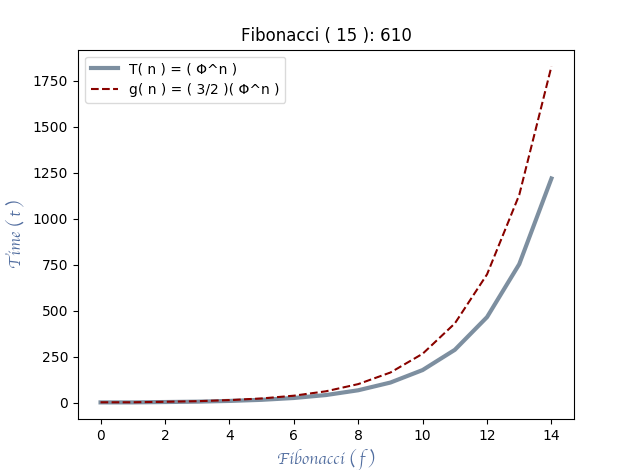
\includegraphics[scale=.4]{gfr2.png}
\centering \linebreak \linebreak Figure 4.2.3: Plot of Figure 4.2.2.
\end{figure}

\begin{center}
\begin{tabular}[.5cm]{l c c }
\toprule
Time ( t ) & Fibonacci ( n ) \\
\midrule
1 & F ( 1 ) = 1 \\
\cmidrule{1-2}
1 & F ( 2 ) = 1 \\
\cmidrule{1-2}
3 & F ( 3 ) = 2 \\
\cmidrule{1-2}
5 & F ( 4 ) = 3 \\
\cmidrule{1-2}
9 & F ( 5 ) = 5 \\
\cmidrule{1-2}
15 & F ( 6 ) = 8 \\
\cmidrule{1-2}
25 & F ( 7 ) = 13 \\
\cmidrule{1-2}
41 & F ( 8 ) = 21 \\
\cmidrule{1-2}
67 & F ( 9 ) = 34 \\
\cmidrule{1-2}
109 & F ( 10 ) = 55 \\
\cmidrule{1-2}
177 & F ( 11 ) = 89 \\
\cmidrule{1-2}
287 & F ( 12 ) = 144 \\
\cmidrule{1-2}
465 & F ( 13 ) = 233 \\
\cmidrule{1-2}
753 & F ( 14 ) = 377 \\
\cmidrule{1-2}
1219 & F ( 15 ) = 610 \\
\bottomrule
\linebreak
\end{tabular}
\linebreak Table 6: Plot points of Figure 4.2.3.
\end{center}
\end{multicols} 

\pagebreak

\subsection{Cube-Sum Iterative:}

First test of the Cubes-Sum Iterative Algorithm. The program will plot the {\bfseries\itshape time} that the algorithm takes to find the sum of the {\bfseries\itshape tenth} first numbers to the power '3', excluding '0'.

\begin{figure}[H]
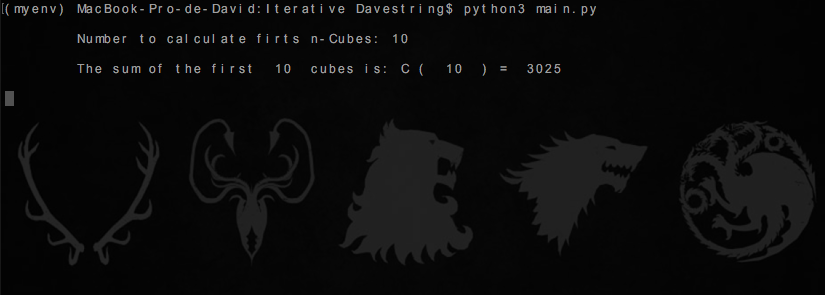
\includegraphics[scale=.6]{cci1.png}
\centering \linebreak \linebreak Figure 4.3.0: Console output of Cubes-Sum Iterative.
\end{figure}

\begin{multicols}{2}
\begin{figure}[H]
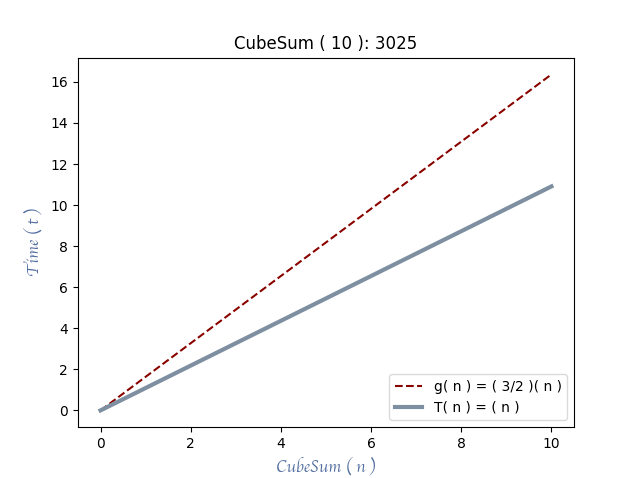
\includegraphics[scale=.4]{gci1.png}
\centering \linebreak \linebreak Figure 4.3.1: Plot of Figure 4.3.0.
\end{figure}

\begin{center}
\begin{itemize}
\end{itemize}
\begin{tabular}[.5cm]{l c c }
\toprule
Time ( t ) & CubeSum ( n ) \\
\midrule
0 & C ( 0 ) = 0 \\
\cmidrule{1-2}
1.2 & C ( 1 ) = 1 \\
\cmidrule{1-2}
2.4 & C ( 2 ) = 9 \\
\cmidrule{1-2}
3.6 & C ( 3 ) = 36 \\
\cmidrule{1-2}
4.8 & C ( 4 ) = 100 \\
\cmidrule{1-2}
6.0 & C ( 5 ) = 224 \\
\cmidrule{1-2}
7.2 & C ( 6 ) = 441 \\
\cmidrule{1-2}
8.4 & C ( 7 ) = 784 \\
\cmidrule{1-2}
9.6 & C ( 8 ) = 1296 \\
\cmidrule{1-2}
10.8 & C ( 9 ) = 2025 \\
\cmidrule{1-2}
12 & C ( 10 ) = 3025 \\
\bottomrule
\linebreak
\end{tabular}
\linebreak Table 7: Plot points of Figure 4.3.1.
\end{center}
\end{multicols}

{\bfseries\itshape\color{OliveGreen}{Observation:}} {\itshape\color{OliveGreen}{The plot has two curves, the {\bfseries blue} one it's the computation time of our algorithm \linebreak {\bfseries T( n ) = n} and the {\bfseries red} one it's the proposed function {\bfseries g( n ) = $\frac{3}{2} n$}, where {\bfseries T( n ) $\in$ O ( g( n ) ).}}} \hfill \break

\pagebreak

\subsection{Cube-Sum Recursive:}

First test of the Cubes-Sum Recursive Algorithm. The program will plot the {\bfseries\itshape time} that the algorithm takes to find the sum of the {\bfseries\itshape tenth} first numbers to the power '3', excluding '0'.

\begin{figure}[H]
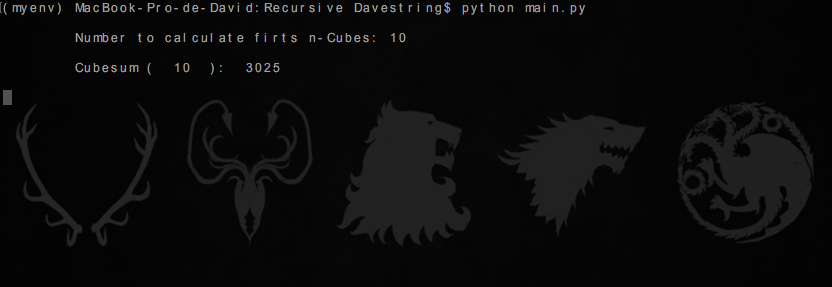
\includegraphics[scale=.6]{ccr1.png}
\centering \linebreak \linebreak Figure 4.4.0: Console output of Cubes-Sum Recursive.
\end{figure}

\begin{multicols}{2}
\begin{figure}[H]
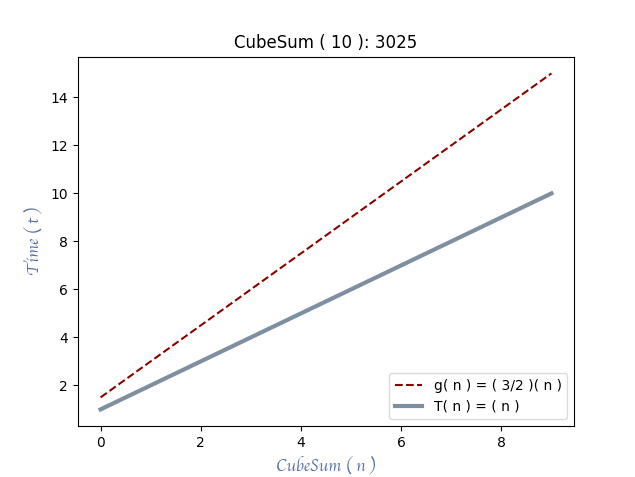
\includegraphics[scale=.4]{gcr1.png}
\centering \linebreak \linebreak Figure 4.4.1: Plot of Figure 4.4.0.
\end{figure}

\begin{center}
\begin{itemize}
\end{itemize}
\begin{tabular}[.5cm]{l c c }
\toprule
Time ( t ) & CubeSum ( n ) \\
\midrule
0 & C ( 0 ) = 0 \\
\cmidrule{1-2}
1 & C ( 1 ) = 1 \\
\cmidrule{1-2}
2 & C ( 2 ) = 9 \\
\cmidrule{1-2}
3 & C ( 3 ) = 36 \\
\cmidrule{1-2}
4 & C ( 4 ) = 100 \\
\cmidrule{1-2}
5 & C ( 5 ) = 224 \\
\cmidrule{1-2}
6 & C ( 6 ) = 441 \\
\cmidrule{1-2}
7 & C ( 7 ) = 784 \\
\cmidrule{1-2}
8 & C ( 8 ) = 1296 \\
\cmidrule{1-2}
9 & C ( 9 ) = 2025 \\
\cmidrule{1-2}
10 & C ( 10 ) = 3025 \\
\bottomrule
\linebreak
\end{tabular}
\linebreak Table 8: Plot points of Figure 4.4.1.
\end{center}
\end{multicols}

{\bfseries\itshape\color{OliveGreen}{Observation:}} {\itshape\color{OliveGreen}{The plot has two curves, the {\bfseries blue} one it's the computation time of our algorithm \linebreak {\bfseries T( n ) = n} and the {\bfseries red} one it's the proposed function {\bfseries g( n ) = $\frac{3}{2} n$}, where {\bfseries T( n ) $\in$ O ( g( n ) ).}}} \hfill \break

\pagebreak

\section{Annexes:}

\subsection{Bubble-Sort Formal Demonstration:}

Calculate the temporal complexity of the Bubble-Sort algorithm: \hfill \break

\begin{lstlisting}
for i = 1 to i <= n - 1 do
	for j = n - 1 to j >= i do
		if ( A [ j ] < A [ j - 1 ] )
			exchange: A [ j ] with A [ j - 1 ]
\end{lstlisting}

\begin{itemize}
\item {\bfseries\itshape\color{CadetBlue}{Where n = A.length:}} \hfill
\end{itemize}

As we can see, the algorithm sort the array {\bfseries\itshape A} in his ascendant form, so, the worst case, it's when the array already it's sorted but in his descendant form.

\begin{itemize}
\item {\bfseries\itshape\color{Maroon}{Solution:}} \hfill
\end{itemize}

\begin{ceqn}
\begin{align}
T ( n ) = C_{1}( n ) + C_{2}[ \sum_{i = 1}^{n - 1} ( t_{i} ) ] + C_{3}[ \sum_{i = 1}^{n - 1} ( t_{i - 1} ) ] + C_{4}
\end{align}
\end{ceqn}

{\bfseries\itshape\color{CadetBlue}{For $t_{i}$:}} \hfill \break

\begin{center}
\begin{tabular}[.5cm]{l c c c }
\toprule
i & $t_{i}$ & range \\
\midrule
1 & n - 1 & n - 1 $\geq$ j $\geq$ 1 \\
\cmidrule{1-3}
2 & n - 2 & n - 1 $\geq$ j $\geq$ 2 \\
\cmidrule{1-3}
3 & n - 3 & n - 1 $\geq$ j $\geq$ 3 \\
\cmidrule{1-3}
- & then & - \\
\cmidrule{1-3}
i & n - i & n - 1 $\geq$ j $\geq$ i\\
\bottomrule
\linebreak
\end{tabular}
\linebreak Table 9: $t_{i}$ value.
\end{center}

{\bfseries\itshape\color{CadetBlue}{Let $t_{i}$ = n - 1, substituting in ( 4 ):}} \hfill \break

\begin{ceqn}
\begin{align}
T ( n ) &= C_{1}( n ) + C_{2}[ \sum_{i = 1}^{n - 1} ( n - i ) ] + C_{3}[ \sum_{i = 1}^{n - 1} ( ( n - 1 ) - i ) ] + C_{4} \\
&= C_{1}( n ) + C_{2}[ \sum_{i = 1}^{n - 1} ( n ) ] - C_{2}[ \sum_{i = 1}^{n - 1} ( i ) ] + C_{3}[ \sum_{i = 1}^{n - 1} ( n - 1 ) ] - C_{3}[ \sum_{i = 1}^{n - 1} ( i ) ] + C_{4}
\end{align}
\end{ceqn}

{\bfseries\itshape\color{CadetBlue}{Using:}} \hfill \break
{\color{CadetBlue}{
\begin{tasks}
\task $\sum_{i = m}^{n} ( k ) = k ( n - m + 1 )\ where\ k\ constant.$
\task $\sum_{i = m}^{n} ( i ) = \frac{(n + 1 - m)( n + m )}{2}. $
\end{tasks}}} \hfill

{\bfseries\itshape\color{CadetBlue}{Then:}} \hfill 

\begin{ceqn}
\begin{align}
T( n ) &= C_{1}( n ) + C_{2}[ n ( n - 1 ) ] - C_{2}[ \frac{( n - 1 )( n )}{2} ] + C_{3}[ ( n - 1 )( n - 1 ) ] - C_{3}[ \frac{( n - 1 )( n )}{2} ] + C_{4} \\
&= C_{1}( n ) + C_{2}[ n^{2} - n ] - C_{2}[ \frac{n^{2} - n}{2} ] + C_{3}[ n^{2} - 2n + 1 ] - C_{3}[ \frac{n^{2} - n}{2} ] + C_{4} \\
&= C_{1}( n ) + C_{2}n^{2} - C_{2}n - C_{2}\frac{n^{2}}{2} + C_{2}\frac{n}{2} + C_{3}n^{2} - 2C_{3}n + C_{3} - C_{3}\frac{n^{2}}{2} + C_{3}\frac{n}{2} + C_{4} \\
&= [ n^{2} ][ C_{2}\frac{1}{2} + C_{3}\frac{1}{2} ] + [ n ][ C_{1} - C_{2}\frac{1}{2} - C_{3}\frac{3}{2}] + [C_{3} + C_{4}] \\
&= an^{2} + bn + c
\end{align}
\end{ceqn}

{\bfseries\itshape\color{CadetBlue}{Finally:}} \hfill 

\begin{ceqn}
\begin{align}
T(\ n\ )\ \in\ \theta (\ n^{2}\ )
\end{align}
\end{ceqn}

\pagebreak

\subsection{Iterative Fibonacci Formal Demonstration:}

Demonstrate that the Fibonacci iterative algorithm has {\bfseries\itshape linear} order:  \hfill \break

\begin{lstlisting}
a, b = 1, 0
for i = 0 to i < n do
	f = a + b
	b = a
	a = f
\end{lstlisting}

\begin{itemize}
\item {\bfseries\itshape\color{Maroon}{Demonstration:}} \hfill
\end{itemize}

\begin{ceqn}
\begin{align}
T( n ) &= C_{1} + C_{2}[ n + 1 ] + C_{3}[ n ] + C_{4}[ n ] + C_{5}[ n ] \\
&= C_{1} + C_{2}[ n ] + C_{2} + C_{3}[ n ] + C_{4}[ n ] + C_{5}[ n ] \\
&= [ n ] [ C_{2} + C_{3} + C_{4} + C_{5} ] + [ C_{1} + C_{2} ]
\end{align}
\end{ceqn}

{\bfseries\itshape\color{CadetBlue}{Substituting: \hfill \break
\begin{tasks}
\task Let a = $C_{2} + C_{3} + C_{4} + C_{5}$.
\task Let b = $C_{1} + C_{2}$.
\end{tasks}}} \hfill

{\bfseries\itshape\color{CadetBlue}{Then:}}

\begin{ceqn}
\begin{align}
T( n ) = an + b
\end{align}
\end{ceqn} \hfill

{\bfseries\itshape\color{CadetBlue}{Finally:}}

\begin{ceqn}
\begin{align}
T(\ n\ )\ \in\ O(\ n\  ).
\end{align}
\end{ceqn}

\pagebreak

\subsection{Iterative Cube-Sum Formal Demonstration:}

Demonstrate that the Cube-Sum iterative algorithm has {\bfseries\itshape linear} order: \hfill \break

\begin{lstlisting}
sum = 0
for i = 1 to i <= n do:
	sum = sum + ( i * i * i )
\end{lstlisting}

\begin{itemize}
\item {\bfseries\itshape\color{Maroon}{Demonstration:}} \hfill
\end{itemize}

\begin{ceqn}
\begin{align}
T( n ) &= C_{1} + C_{2}( n + 1 ) C_{3}( n ) \\
&= [ n ] [ C_{2} + C_{3} ] + [ C_{1} + C_{2} ] 
\end{align}
\end{ceqn}

{\bfseries\itshape\color{CadetBlue}{Substituting: \hfill \break
\begin{tasks}
\task Let a = $C_{2} + C_{3}$.
\task Let b = $C_{1} + C_{2}$.
\end{tasks}}} \hfill

{\bfseries\itshape\color{CadetBlue}{Then:}}

\begin{ceqn}
\begin{align}
T( n ) = an + b
\end{align}
\end{ceqn} \hfill

{\bfseries\itshape\color{CadetBlue}{Finally:}}

\begin{ceqn}
\begin{align}
T(\ n\ )\ \in\ O(\ n\  ).
\end{align}
\end{ceqn}

\pagebreak

\subsection{Recursive Cube-Sum Formal Demonstration:}

Demonstrate that the Cube-Sum recursive algorithm has {\bfseries\itshape linear} order: \hfill \break

\begin{lstlisting}
if ( n == 1 ) return 1
else return S ( n - 1 ) + n*n*n
\end{lstlisting}

\begin{ceqn}
\begin{align}
M( n ) = \left\{
\begin{array}{ll}
1 & \mathrm {if\ } n = 1 \\
M(n-1) + 1 & \mathrm {if\ } n > 1 \\
\end{array}
\right.
\end{align}
\end{ceqn} 

\begin{itemize}
\item {\bfseries\itshape\color{Maroon}{Demonstration:}} \hfill
\end{itemize}

\begin{ceqn}
\begin{align} 
M ( n ) &= M ( n - 1 ) + 1  \\
&= [\ M ( n - 2 ) + 1\ ] + 1 \\
&= [\ (\ M ( n - 3 ) +1\ ) + 1\ ] + 1 \\
&= [\ (\ (\ M ( n - 4 ) + 1\ ) + 1\ ) + 1\ ] + 1 \\ 
\end{align}
\end{ceqn}

{\bfseries\itshape\color{CadetBlue}{So on:}}

\begin{ceqn}
\begin{align} 
M ( n ) &= M ( n - i ) + i 
\end{align}
\end{ceqn}

{\bfseries\itshape\color{CadetBlue}{Substituting: \hfill \break
\begin{tasks}
\task n - i = 1.
\task i = n - 1.
\end{tasks}}} \hfill

{\bfseries\itshape\color{CadetBlue}{then:}}

\begin{ceqn}
\begin{align}
M(\ n\ ) &= M (1) + ( n - 1 ) \\
\end{align}
\end{ceqn}

{\bfseries\itshape\color{CadetBlue}{Finally:}}

\begin{ceqn}
\begin{align}
M(\ n\ )\ \in\ O(n).
\end{align}
\end{ceqn}

\pagebreak

\section{Conclusion:}

As we have seen up to this point in our career, there are many forms to solve the same problem. We where analyzing the Fibonacci algorithm in this practice using a {\bfseries\itshape recursive} and a {\bfseries\itshape iterative} code. But they aren't the only ways to solve this problem, in {\bfseries practice 1} I wrote the Fibonacci algorithm using a {\bfseries\itshape generator}, and also I know we can use {\bfseries\itshape memories} to help optimize the algorithm. At the end, we as programmers will use the one who solve the problem better, using the computer resources optimally, and all our knowledge gained over this time. It's quite interesting see that, apart of being the same problem solved in two different ways, the graph of the recursive algorithm vs the iterative are very different because of the time that our computer takes to solve the same problem.

\begin{flushright}
- Hernandez Martinez Carlos David.
\end{flushright} \hfill

Sometimes we think that the recursion is better than iterative algorithm, in this case we demonstrate that this premise is not always true, because there are variables in the environmental development that influences in the computational time like hardware, memory, cores, processors, etc. The recursion is a way to solve problems but in code is not  always the better solution, sometimes the  lines of code is higher than the other one and therefore many times the constants of time grow in number, I think recursion is better in the cases when the complex of the development "code" is bigger, the best way to have an idea of what kind of algorithm implementation is better than the other is to calculate the order complexity.

\begin{flushright}
- Burciaga Ornelas Rodrigo Andres.
\end{flushright}

\pagebreak

\section{Bibliography References:}

[ 1 ] Baase and Van Gelder. "Computer Algorithms: Introduction to Design and Analysis". Addison-Wesley. \hfill \break \break
[ 2 ] Thomas H. Cormen. "Introduction to Algorithms". The MIT press.

\end{document}